%!TEX program = pdflatex
\documentclass{article}
\usepackage{graphicx} % Required for inserting images
\usepackage{amsmath}
\usepackage{amssymb}
\usepackage[italian]{babel}
\usepackage{color} % Necessario per gestire i colori
\usepackage[colorlinks=true, linkcolor=blue, urlcolor=blue, citecolor=blue]{hyperref}
\usepackage{booktabs}
\usepackage{xcolor}
\usepackage{colortbl}

\title{Transformers}
\author{Alessandro Ferri}
\date{July 2026}

\begin{document}

\maketitle
{
\hypersetup{linkcolor=black}
\tableofcontents
}
\newpage

\section{Perché sono nati i Transformers? I limiti delle architetture precedenti}
\subsection{Reti Ricorrenti}
Le \textbf{RNN(Recurrent Neural Networks)} e le \textbf{LSTM(Long Short-Term Memory)} sono due tipi di reti neurali che pongono una "base storica" per la nascita dei \textbf{Transformers}.
Sebbene però queste due architetture abbiano introdotto il concetto di \texttt{memoria}, presentano dei limiti nella scalabilità e nelle dipendenze a lungo raggio.

A differenza delle reti Feed-Forward, una RNN elabora una sequenza in input mantenendo uno stato nascosto $h_t$ il quale funge da memoria del contesto.
Il limite di questa architettura però riguarda la sua elaborazione sequenziale, cioè per calcolare lo stato $h_t$ è necessario aver completato il calcolo di $h_{t-1}$, di conseguenza questo approccio non è parallelizzabile, rendendolo così inefficiente.
\subsection{Il Vanishing Gradient}
L'elaborazione in sequenza porta inoltre al problema del \textbf{Vanishing Gradient}, responsabile della perdita di contesto a lungo raggio.

Il Vanishing Gradient avviene quando la correzione degli errori diventa così piccola durante l'addestramento da impedire ai primissimi livelli di imparare.
Questo avviene poiché la rete per capire quanto ogni singolo pezzo della rete ha contribuito all'errore utilizza la \textbf{Backpropagation}, il cui risultato è dato dalla moltiplicazione di molti piccoli numeri (le derivare dei diversi passaggi).
Nelle RNN inizialmente come funzione di attivazione veniva utilizzata la Sigmoide (la cui derivata vale al massimo $0.25$), poiché la moltiplicazione continua di numeri $<1$ tende a $0$, i primi livelli della rete avevano un "assegnazione di colpa" quasi pari a $0$
facendo credere (erroneamente) alla rete che quei livelli funzionano correttamente.
Esiste anche il problema inverso, cioè l'\textbf{Exploding Gradient}, il gradiente che tende ad $+\infty$.

\subsection{Dalle LSTM ai Transformers}
Le architetture \textbf{LSTM} hanno attenuato il problema del vanishing gradient tramite l'introduzione dei gate (gate di input, forget ed output).
Rimane però il problema dell'elaborazione sequenziale.
Inoltre la distanza che l'informazione deve attraversare tra due token distanti $L$ è di ordine $O(L)$.
I transformer eliminano queste problematiche tramite l'introduzione del meccanismo della \textbf{Self-Attention}, permettendo l'elaborazione simultanea di tutti i token in input, rendendo inoltre la distanza di ogni coppia di token di ordine $O(1)$


\section{Il meccanismo della Self Attention}
\subsection{Cos'è e come si ottengono Q, K, V}
\label{sec:vettori}
La \textbf{Self Attention} è un meccanismo che permette al modello di mettere in relazione due o più parole di una singola frase.
Per fare ciò il modello ricava 3 vettori per ogni parola nella frase.
Dato un input $X$ (che rappresenta la sua matrice di embedding di partenza, di dimensione
$L \times d_{model}$, dove $L$ è la grandezza della sequenza e $d_{model}$ è la dimensione del modello)
il modello non lavora direttamente su $X$, ma calcola delle nuove rappresentazioni tramite proiezioni lineari.
Quest'ultime sono ottenute moltiplicando l'input per 3 matrici di pesi derivate dall'addestramento del modello, chiamate $W^Q$, $W^K$ e $W^V$.
\begin{itemize}
    \item \textbf{Query($Q=XW^Q$)}: Rappresenta cosa sta cercando la parola \textbf{attuale} che il modello sta analizzando. Può essere interpretata come la domanda che il token pone agli altri elementi per comprendere le proprie dipendenze grammaticali, sintattiche o semantiche nel contesto.
    \item \textbf{Key($K=XW^K$)}: Rappresenta le "caratteristiche" di una determinata parola, cioè a quale tipo di ricerca può rispondere; viene infatti confrontata con tutte le Query per calcolare i punteggi di affinità tra le varie parole.
    \item \textbf{Value($V=XW^V$)}: Rappresenta il valore effettivo della parola, la quale servirà per creare la rappresentazione contestualizzata della parola. Ad esempio se la compatibilità tra la Query di un token $A$ e la Key di un token $B$ risulta elevata, il vettore Value del token $B$ contribuirà in modo massiccio alla costruzione della nuova rappresentazione di $A$, cioè $A$ assorbirà il contesto di $B$
\end{itemize}

Le matrici $W^Q$ e $W^K$ proiettano l'input in uno spazio di dimensione $d_k$, invece $W^V$ proietta in uno spazio di dimensione $d_v$.
Questa distinzione è dovuta al fatto che la formula per il calcolo delle affinità (che come vedremo è $QK^T$) obbliga i due vettori a trovarsi nello stesso spazio vettoriale,
mentre il vettore Value è libero di essere in uno spazio diverso (anche se nella pratica spesso $d_k=d_v$).



Questi vettori consentono al modello di calcolare i \textbf{punteggi di attenzione}, determinando il grado di affinità di ogni parola verso le altre parole, permettendo al modello di capire il contesto.

Facciamo un esempio per capire cosa fa la self-attention concretamente.
Immaginiamo di avere la frase \newline
\texttt{il tecnico ha configurato la rete per connettere i computer.} \newline
Un umano può facilmente presumere dal contesto che la parola \texttt{rete} sia legata ad un concetto di telecomunicazioni, e non ad una rete da pesca.
La Self-Attention risolve proprio questo problema, quando il meccanismo valuterà la parola "rete" tramite la sua Query troverà un'altissima affinità con le parole "tecnico", "configurato" e "computer",
questo permetterà alla nuova rappresentazione risultante di integrare le informazioni provenienti da quelle parole.

\subsection{Come funziona}
\label{sec:formula-attention}

La formula che governa la self-attention è la seguente:
$$
\text{Attention}(Q, K, V) = \text{softmax}\left(\frac{Q K^T}{\sqrt{d_k}}\right) V 
$$
Dividiamo il suo calcolo in 4 step: \newline
\textbf{Step 1: Calcolo delle affinità $QK^T$}: Si calcola l'affinità della parola in esame, quella nella query, con tutte le altre parole all'interno della frase. Questo avviene tramite prodotto scalare delle matrici, la matrice risultante conterrà i punteggi di attenzione grezzi, dove la cella $(i,j)$ indica l'affinità tra la Query dell'i-esimo token e la Key dei j-esimo token, il quale avrà un valore alto se due parole hanno alta affinità e un valore basso altrimenti. \newline
\textbf{Step 2: La stabilizzazione $\sqrt{d_k}$}: Questo passaggio va semplicemente a scalare i numeri per fare in modo di non lavorare con numeri enormi, i quali potrebbero poi essere un problema per il calcolo del gradiente, dove $d_k$ è la dimensione del vettore Key \newline
\textbf{Step 3: La normalizzazione in percentuale, funzione Softmax}: A questo punto alla matrice viene applicata la funzione \textbf{Softmax}, producendo $$A = \text{softmax}\left(\frac{Q K^T}{\sqrt{d_k}}\right)$$ 
La matrice $A \in \mathbb{R}^{L \times L}$ contiene quindi i nostri \textbf{pesi di attenzione}, poiché la funzione softmax per ogni riga $i$ mappa i punteggi grezzo in un distribuzione di probabilità, infatti per le proprietà delle distribuzioni: $$\sum_{j=1}^{L} A_{i, j} = 1 \quad \text{con } A_{i, j} \in [0, 1]$$ Quindi in modo simile a prima $A[i,j]$ quantifica la percentuale di "attenzione" che il token $i$ deve assegnare al token $j$.
\textbf{Step 4: Estrazione del significato $\times V$}: Infine la matrice con i pesi di attenzione viene moltiplicata per la matrice Value $V$, ciò vuol dire che l'output per il token $i$ è la media pesata di tutti i vettori Value della sequenza: $$\text{Output}_i = \sum_{j=1}^{L} A_{i, j} V_j$$
A questo punto il vettore risultante del token $i$ conterrà sia il suo significato originale, sia il contesto (in modo pesato) derivante da tutti gli altri token.

Riprendiamo ora l'esempio fatto in precedenza per capire come funziona il meccanismo.
\begin{enumerate}
    \item \textbf{Calcolo delle affinità}: La Query associata alla parola "rete" viene confrontata con le Key di tutte le altre parole, producendo i punteggi grezzi: $$e_{\text{rete}, j} = \frac{q_{\text{rete}} \cdot k_j^T}{\sqrt{d_k}}$$ dove $e_{\text{rete}, j}$ indica il punteggio tra la parola "rete" e la j-esima parola della frase 
    \item \textbf{Normalizzazione}: La funzione Softmax trasforma i punteggi grezzi in una distribuzione di probabilità $\alpha_{\text{rete}, j}$ (le quali formano la matrice $A$ della spiegazione precedente), per esempio: 
    \begin{itemize}
        \item $\alpha_{\text{rete}, \text{computer}} \approx 0.45$
        \item $\alpha_{\text{rete}, \text{configurato}} \approx 0.30$
        \item $\alpha_{\text{rete}, \text{tecnico}} \approx 0.15$
        \item $\alpha_{\text{rete}, \text{il/la/per}} \approx 0.03 \dots 0.05$
    \end{itemize} 
    \begin{table}[ht]
    \centering
    \small
    \begin{tabular}{lcccccccc}
    \toprule
    \textbf{Query ($Q$)} & \multicolumn{8}{c}{\textbf{Pesi di Attenzione rispetto alle Key ($K$)}} \\
    \cmidrule(lr){2-9}
    & \textit{Il} & \textit{tecnico} & \textit{ha} & \textit{configurato} & \textit{la} & \textit{rete} & \textit{per} & \textit{computer} \\
    \midrule
    \textit{Il}          & 0.05 & 0.85 & 0.02 & 0.03 & 0.01 & 0.02 & 0.01 & 0.01 \\
    \textit{tecnico}     & 0.02 & 0.10 & 0.03 & 0.55 & 0.01 & 0.20 & 0.02 & 0.07 \\
    \textit{ha}          & 0.01 & 0.15 & 0.04 & 0.70 & 0.01 & 0.05 & 0.01 & 0.03 \\
    \textit{configurato} & 0.01 & 0.30 & 0.05 & 0.05 & 0.02 & 0.40 & 0.02 & 0.15 \\
    \textit{la}          & 0.01 & 0.01 & 0.01 & 0.02 & 0.03 & 0.90 & 0.01 & 0.01 \\
    \rowcolor{gray!15} 
    \textbf{\textit{rete}} & \textbf{0.01} & \textbf{0.15} & \textbf{0.01} & \textbf{0.30} & \textbf{0.02} & \textbf{0.06} & \textbf{0.01} & \textbf{0.44} \\
    \textit{per}         & 0.01 & 0.02 & 0.01 & 0.20 & 0.01 & 0.15 & 0.05 & 0.55 \\
    \textit{computer}    & 0.01 & 0.10 & 0.01 & 0.25 & 0.01 & 0.50 & 0.02 & 0.10 \\
    \bottomrule
    \end{tabular}
    \caption{Forma tabellare delle distribuzioni di probabilità prodotte dalla funzione Softmax}
    \label{tab:attention_matrix}
\end{table}
    \item \textbf{Unione contesto}: Infine il nuovo vettore $z_{rete}$ che rappresenterà la parola "rete" è dato dalla combinazione lineari di tutti i Value: $$z_{\text{rete}} = \sum_{j} \alpha_{\text{rete}, j} \, v_j = 0.45 \, v_{\text{computer}} + 0.30 \, v_{\text{configurato}} + 0.15 \, v_{\text{tecnico}} + \dots$$
\end{enumerate}


\subsection{Multi-Head Attention}
Una singola operazione di Self-Attention fatica a catturare contemporaneamente tutte le diverse sfumature di una frase (grammaticali, semantiche, logiche). Per superare questo limite, i Transformer utilizzano la \textbf{Multi-Head Attention}. 
Invece di eseguire una sola operazione di calcolo dell'attenzione con vettori di dimensione $d_{model}$, proietta $h$ volte (dove $h$ è il numero di teste) $Q,K$ e $V$, avendo così proiezioni differenti per ogni testa.

La Multi-Head Attention è definita come: 
$$\text{MultiHead}(Q, K, V) = \text{Concat}(\text{head}_1, \dots, \text{head}_h) W^O$$
dove semplicemente ogni singola testa calcola la propria attenzione sul suo sottospazio, avendo per ogni testa diversi vettori $Q,K,V$
$$\text{head}_i = \text{Attention}\left(Q W_i^Q, K W_i^K, V W_i^V\right)$$

Il vettore $W^O$ ricavato dall'addestramento serve per poter fondere tra loro le informazioni ricavate dalle varie teste, poiché con il semplice \texttt{concat} sono dati messi uno accanto all'altro

Questa strategia mantiene il \textbf{costo computazionale} invariato, poiché nelle implementazioni standard si pone $d_k = d_v = \frac{d_{model}}{h}$.
Ciò vuol dire che, con $d_{model} = 512$ e $h = 8$, ogni testa lavora su sottospazi di dimensione $d_k = 64$.

Lo scopo di questo meccanismo è proiettare, per ogni testa, i token in un diverso spazio di rappresentazione; questo permette ad una testa di capire le dipendenze sintattiche, ad un'altra di riuscire a collegare un pronome ad un soggetto introdotto diverse frasi prima e così via.

\section{L'architettura dei Transformers}
\subsection{Positional Encoding}
\subsubsection{Il problema}
Prima di poter fare qualsiasi calcolo il modello deve trasformare il testo "grezzo" in numeri, per fare ciò effettua quella che prende il nome di \textbf{tokenizzazione}. Il modello spezza il testo in \textbf{token}, i quali possono essere parole intere oppure frammenti di esse, dopodiché assegna un ID univoco ad ognuno di questi token. Successivamente prende l'ID del token e lo converte in un vettore di numeri chiamato \textbf{Embedding}, è proprio il vettore dal quale vengono ricavati Q, K, V di cui parlavamo in \ref{sec:vettori}. Gli Embedding sono una trasformazione del singolo token in una lista di numeri (quindi un vettore), la quale non è casuale ma viene imparata dalla rete leggendo milioni di testi, in modo che parole molto simili (o che appaiono spesso negli stessi contesti) abbiano valori numerici molto simili.

A questo punto sorge il problema, dato che i Transformers leggono tutti i vettori \textbf{contemporaneamente} perdono completamente il concetto di sequenza e ordine delle parole, il \textbf{positional encoding} è nato proprio per risolvere questo.

\subsubsection{La soluzione}
Il \textbf{Positional Encoding} è una tecnica che permette di aggiungere informazione riguardo la posizione di ogni token nella sequenza, la più famosa prende il nome di \textbf{Sinusoidal Positional Encoding} derivato dal suo uso delle funzioni seno e coseno.
Per ogni posizione $pos \in \{0,\dots,L-1\}$ viene generato un vettore $PE_{pos}$ avente la stessa dimensione dell'embedding del token, in modo da poter essere sommato a quest'ultimo:
$$PE_{(pos, \, 2i)} = \sin\left(\frac{pos}{10000^{2i / d_{model}}}\right)$$
$$PE_{(pos, \, 2i+1)} = \cos\left(\frac{pos}{10000^{2i / d_{model}}}\right)$$
dove $pos$ è la posizione del token nella sequenza e $i$ è l'indice del vettore.
La proprietà di questa formula è che le prime dimensioni del vettore $PE$ cambiano ad altissima frequenza al variare della posizione, invece le ultime dimensioni variano su "scale lunghe" (ad esempio cambio di paragrafi),
questa metodologia permette al modello di stare al passo anche con contesti lontani tra loro all'interno di un testo.


\subsection{Encoder}
L'encoder è un componente della rete il cui compito è quello di ricevere in input le rappresentazioni numeriche delle parole (gli embeddings) e trasformarli in embedding contestualizzati, applicando il meccanismo di self-attention e una parte di feed forward.
Il blocco dell'encoder è formato da 6 livelli identici, composti da una parte di self-attention ed una piccola rete neurale feed-forward.
\begin{figure}[h!]
    \centering
    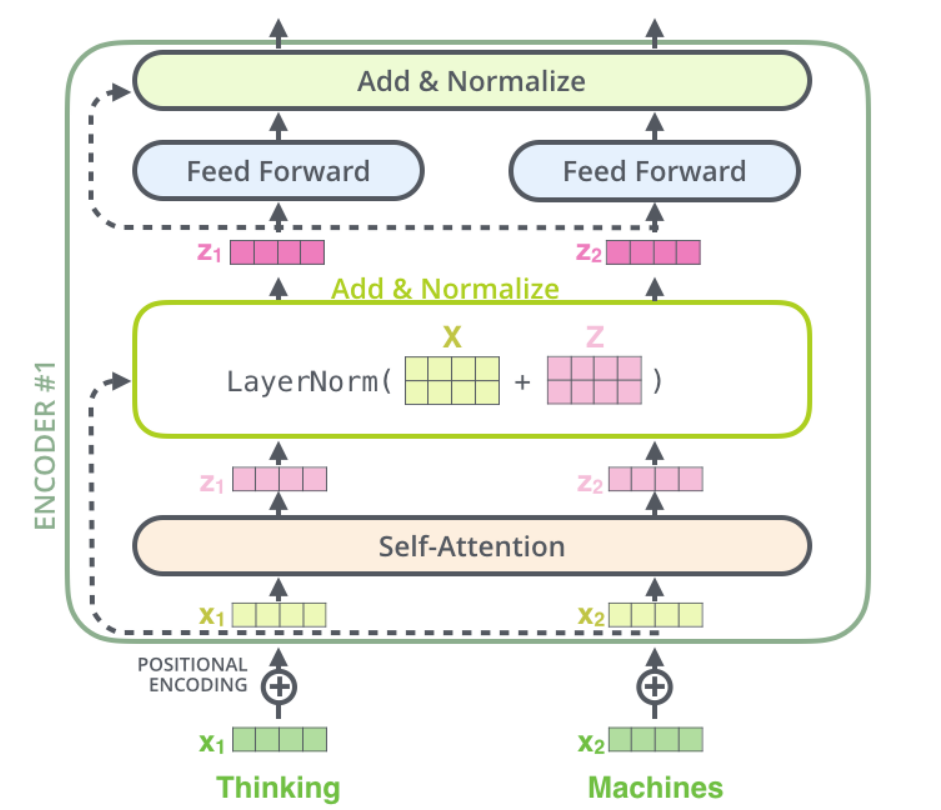
\includegraphics[width=1\textwidth]{img/encoder.png}
    \caption{Struttura di un livello dell'Encoder}
    \label{fig:placeholder}
\end{figure}
Più il dato sale questi livelli, più il modello è in grado di comprendere concetti complessi, ad esempio tramite il primo livello è in grado di capire relazioni semplici (come relazione tra aggettivo e sostantivo) e arrivando all'ultimo può capire il significato globale della frase.
\subsubsection{Applicazione Self-Attention}
Tutto questo avviene in diverse fasi, come possiamo notare dall'immagine l'input iniziale sono i vettori che rappresentano le parole del nostro testo (o comunque la loro divisone in token), con l'aggiunta dell'informazione della posizione. 
A questi vettori viene applicato il meccanismo di self-attention come spiegato nei paragrafi precedenti. 
Dopodiché troviamo il blocco \texttt{Add \& Normalize} il quale ha due compiti:
\begin{enumerate}
    \item \textbf{La parte "Add"}: somma il vecchio vettore $x$ con il risultato del calcolo dell'attenzione, quindi $x+Attention(x)$; questo fa in modo che il modello non elimini l'informazione iniziale del vettore, e in questo modo se uno strato non ha nulla di utile da aggiungere può far passare il vettore $x$ inalterato.
    \item \textbf{La parte "Normalize"}: poiché dopo aver sommato i vettori i numeri potrebbero diventare difficili da gestire (alcuni troppo grandi e altri troppo piccoli), questo strato li riscala in modo che abbiamo media 0 e deviazione standard 1, permettendo alla rete di eseguire l'addestramento in modo omogeneo.
\end{enumerate}
Il blocco \texttt{Add \& Normalize} serve per far sì che il modello non "dimentichi" l'identità base delle parole, semplicemente somma il vettore originale con quello risultante dalla self-attention, applicando infine una normalizzazione.

\subsubsection{Feed-Forward Network}
\label{sec:ffn}
Durante la fase di self-attention ogni token ha assorbito informazioni da ogni altro token, ma alcune di esse potrebbero essere semplice rumore, o potrebbero essere ridondanti; il compito della rete Feed-Forward è elaborare in modo \textbf{indipendente} ogni token e filtrare queste informazioni, in modo da lasciare solo ciò che serve davvero.
Ad esempio durante la Self-Attention la parola "mela" avrà una forte affinità con la parola "mangiato", la Feed-Forward riceverà il vettore contestualizzato e tramite dei suoi pattern interni può legare quel vettore al contesto della nutrizione.

Formalmente, per ciascun vettore $z \in \mathbb{R}^{d_{model}}$:
$$\text{FFN}(z) = \max(0, \, z W_1 + b_1) W_2 + b_2$$
dove:
\begin{itemize}
    \item $W_1 \in \mathbb{R}^{d_{model} \times d_{ff}}$ e $b_1 \in \mathbb{R}^{d_{ff}}$ servono ad espandere la dimensione del vettore (solitamente si quadruplica), permettendo alla rete di avere più dimensioni in cui combinare la feature risultanti dalla self-attention, di conseguenza sarà in grado di trovare relazioni più complesse.
    \item  $W_2 \in \mathbb{R}^{d_{ff} \times d_{model}}$ e $b_2 \in \mathbb{R}^{d_{model}}$ invece riportano il vettore alla sua dimensione originale, in modo da filtrare il rumore accumulato durante l'espansione del vettore, in questo modo rimarranno solamente pattern rilevanti.
\end{itemize}
\subsection{Decoder}

L'ultimo pezzo è il \textbf{decoder}, il quale prenderà tutta la conoscenza generata dall'\textbf{encoder} per generare un risposta (ad esempio una traduzione).
A differenza dell'encoder il quale legge tutto il testo in un colpo solo, il decoder genera una parola alla volta (\textbf{autoregressione}). Anche per il decoder abbiamo una struttra a livelli, ma questa volta dentro ogni livello è presente un meccanismo aggiuntivo, avendone in tutto 3.

\subsubsection{Masked Self-Attention}
\label{masked}
A differenza dell'Encoder, il quale può osservare l'intera sequenza in entrambe le direzioni, il Decoder non può osservare le informazioni dei token successivi a quello che sta predicendo.
Questo poiché altrimenti il modello durante l'addestramento "sbircerebbe" le parole successive e le andrebbe a copiare invece di effettuare una previsione.
Per fare ciò si applica il meccanismo che prende il nome di \textbf{Masked Self-Attention} durante il calcolo dell'attenzione.
$$\text{MaskedAttention}(Q, K, V) = \text{softmax}\left(\frac{Q K^T}{\sqrt{d_k}} + M\right) V$$
La formula è quasi uguale a quella definita in \ref{sec:formula-attention}, con l'aggiunta della matrice di mascheramento $M \in \mathbb{R}^{L \times L}$ definita come:
$$M_{i, j} = \begin{cases} 0 & \text{se } j \le i \\ -\infty & \text{se } j > i \end{cases}$$
In questo modo alle posizioni successive a quella attuale viene sommato $-\infty$, il quale verrà portato a 0 dalla funzione Softmax.

Facciamo un piccolo esempio per capire qual è il risultato:
consideriamo la generazione della frase \texttt{[BOS] Il gatto dorme} ([BOS] indica l'inizio della frase).
La matrice dei punteggi grezzi derivante dall'addestramento è la seguente
$$S = \frac{QK^T}{\sqrt{d_k}} =  \begin{pmatrix} s_{11} & s_{12} & s_{13} & s_{14} \\ s_{21} & s_{22} & s_{23} & s_{24} \\ s_{31} & s_{32} & s_{33} & s_{34} \\ s_{41} & s_{42} & s_{43} & s_{44} \end{pmatrix}$$
Applicando la matrice $M$ otteniamo
$$S + M =  \begin{pmatrix} s_{11} & -\infty & -\infty & -\infty \\ s_{21} & s_{22} & -\infty & -\infty \\ s_{31} & s_{32} & s_{33} & -\infty \\ s_{41} & s_{42} & s_{43} & s_{44} \end{pmatrix}$$
Applicando la funzione Softmax i $-\infty$ verranno trasformati in $0$.
In questo modo il funzionamento è il seguente:
\begin{itemize}
    \item Nella riga 1 il modello deve predire "Il" potendo guardare solo il token [BOS]($s_{11}$) e non le parole successive
    \item Nella riga 2 deve predire "gatto" potendo guarda solo [BOS]($s_{21}$) e "Il"($s_{22}$) e non la parole successive e così via
\end{itemize}
\subsubsection{Encoder-Decoder Attention}
A questo punto avviene la "connessione" tra Encoder e Decoder, permettendo a quest'ultimo di guardare solo ciò che è rilevante della sequenza in input.
La formula è identica a quella della Multi-Head Attention, l'unica differenza è che le Query appartengono al Decoder, rappresentando ciò che il decoder deve generare al passo corrente; 
Key e Value invece provengono dall'Encoder, rappresentando in modo completo e contestualizzato la frase in input.
Ogni volta che il Decoder dovrà generare una parola andrà a confrontare la sua Query con le Key e Value dell'Encoder per capire su quali token dover concentrare l'attenzione.
\subsubsection{Feed-Forward Network e generazione dell'output}
A questo punto il vettore passa per una Feed-Forward Network identica a quella descritta in \ref{sec:ffn}.
Dopodiché inizia la fase in cui il vettore $h_{\text{out}} \in \mathbb{R}^{d_{model}}$ risultante dalla FFN viene trasformato in token:
\begin{enumerate}
    \item Il vettore viene proiettato nello spazio del vocabolario, un vocabolario interno del modello composto da tutte le parole di sua conoscenza.
    $$\text{logits} = h_{\text{out}} W_{\text{vocab}} + b_{\text{vocab}}$$
    dove $W_{\text{vocab}} \in \mathbb{R}^{d_{model} \times \vert{}V\vert{}}$ e $\vert{}V\vert{}$ è la dimensione del vocabolario. Con questo passaggio otteniamo un vettore di punteggi grezzi.
    \item Infine tramite la funzione Softmax trasformiamo i punteggi grezzi in distribuzioni di probabilità, selezionando (o con una Greedy Search o con altri algoritmi) il token da generare come parola successiva.
\end{enumerate}



\section{I diversi tipi di Transformers}
\subsection{Encoder-Only}
I modelli \textbf{Encoder-Only} sono formati, come dice il nome, solamente dal meccanismo dell'encoder, questo gli permette di essere specializzati nel \textbf{comprendere a fondo} un testo con tutto il suo contesto.
Questi modelli calcolano la Self-Attention in modo bidirezionale, hanno quindi accesso al contesto sia a sinistra che a destra, senza meccanismi di masking.
Durante il loro addestramento alcuni token vengono sostituiti da un token speciale ([MASK]), in questo modo la rete sarà costretta ad indovinare quei token permettendogli di assorbire un contesto più profondo.
Questi modelli sono ottimi per \textbf{classificazione di testo, estrazione di feature ecc.}

\subsection{Decoder-only}
Al contrario, i \textbf{Decoder-Only} (ad es. chatGPT) vantano solo la componente del decoder, questo li rende specializzati nel \textbf{"prevedere il futuro"}, per esempio generazione di testi.

A differenza degli Encoder-Only, questi non possono vedere l'intera sequenza per i motivi spiegati precedentemente, di conseguenza il modello viene addestrato mantenendo la Masked Self-Attention (\ref{masked})

\subsection{Encoder-Decoder}
Gli \textbf{Encoder-Decoder} invece sono il modello originale, costituiti da entrambi i meccanismi appena visti.
Vengono utilizzati ad esempio per \textbf{traduzioni e riassunti}
\end{document}
